Vortex core lines describe the centers of swirling behavior in vector fields.
%
They are a useful tool in vector field visualization because they provide an
explicit geometrical representation of an important flow feature.
%
Different definitions and strategies for extracting vortex core lines have been
presented in \cref{sub:vortex_extraction}.
%
One of the simplest and most popular methods is the one proposed by Sujudi and
Haimes~\cite{Sujudi1995}, which can be computed using the \ac{PV}
operator~\cite{Peikert1999}.
%

%
Tensor field lines, \ie, lines that are everywhere tangential to an eigenvector
of a tensor field (see \cref{sub:tensor_line_surface_based}), can also exhibit
``swirling'' behavior similar to vortices in vector fields.
%
For example, stress tensor fields show stress trajectories winding around a
common core in regions of twist.
%
Various visualization methods for tensor fields exist, but to date no approach
has been proposed to extract core lines of such vortex-like structures.
%

%
As we have already explained in \cref{cha:parallel_eigenvectors}, simply using
the Sujudi/Haimes criterion and applying the \ac{PV} operator to the
``eigenvector fields'' of the data cannot give consistent results.
%
We therefore introduce \emph{tensor core lines} as an equivalent to vortex
core lines in vector fields.
%
Their definition is a direct extension of the Sujudi/Haimes criterion to tensor
fields and their extraction is based on the \ac{PEV} operator.
%
\begin{figure}[t]
    \centering
    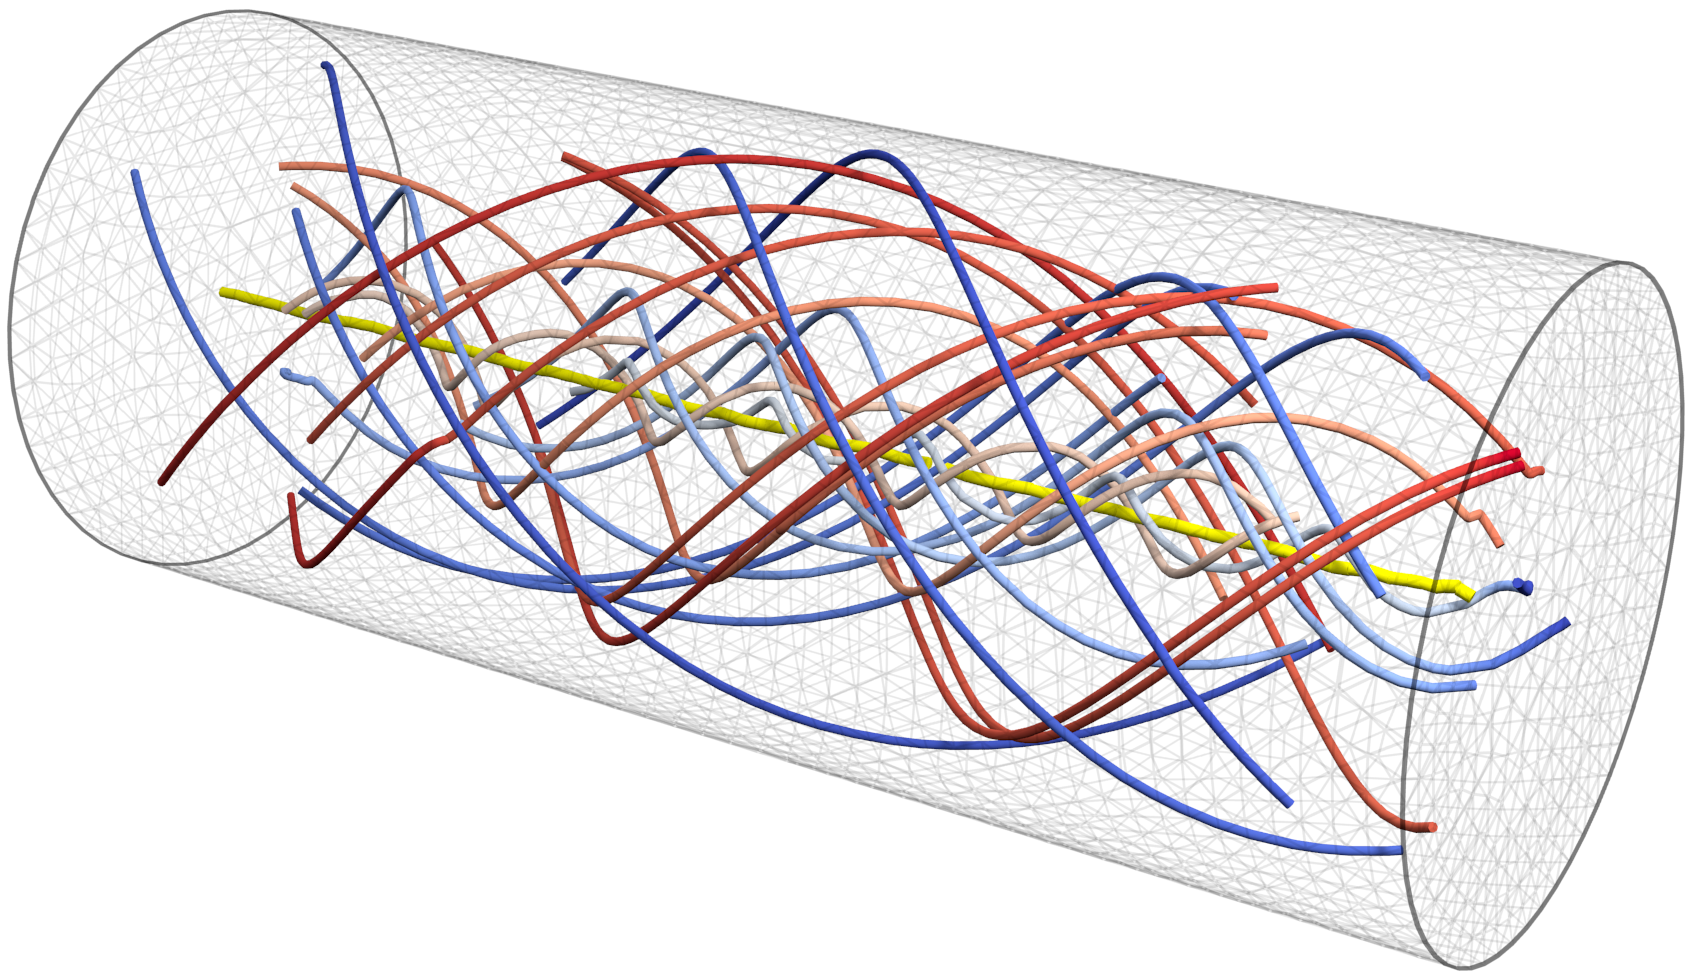
\includegraphics[width=\columnwidth]{figures/torque_tube_lines.png}
    \caption{Eigenvector trajectories in a stress tensor field induced by
             applying a torque to a cylindrical shaft. Trajectories of both
             major (blue) and minor (red) eigenvectors show a swirling behavior
             around a common core line (yellow).
             \Todo[inline]{Add arrows to indicate twist}}
    \label{fig:tube_lines}
\end{figure}
%
In particular, we make the following contributions:
%
\begin{itemize}
    \item  We give a rigorous definition of tensor core lines and show that
    indeed the definition gives structurally stable line structures.
    %
    \item We provide a numerical algorithm for the extraction of tensor core
    lines from piecewise linear tensor fields.
    %
    \item We introduce a filter criterion based on numerical stability to
    separate significant and insignificant tensor core lines.
    %
    \item We show tensor core lines in mechanical stress tensor fields,
    interpret them and compare them with degenerate lines where two eigenvalues
    are equal.
\end{itemize}
%
We introduce tensor core lines in \cref{sec:tcl_theory} and study their
properties.
%
We then present our algorithm for extracting tensor core lines in
\cref{sec:extracting_tensor_lines}.
%
We show our results on several stress tensor fields in \cref{sec:tcl_results}
and study the performance, robustness and relation to degenerate lines.
%
As it turns out, our algorithm is sufficiently generic to be applied to the
extraction of \ac{PEV} lines and degenerate lines as well.
%
We show how this can be done in \cref{sec:computing_pev_and_degenerate_lines}
and close with a discussion in \cref{sec:tcl_discussion}.
%
% section introduction (end)